\chapter{Анализ модели Дирихле}

\section{Математическое ожидание числа циклов заданной длины}
Одним из самых важных параметров модели является число циклов заданной длины.
Для простоты изложения сначала будут рассмотрены циклы с конкретными и малыми длинами ($1$ и $2$).
Далее эти рассуждения будут обобщены на циклы произвольной длины $m$.

\subsection{Подсчет циклов длины один}
Для начала оценим число циклов единичной длины.
То есть это либо те циклы, которые не были затронуты в марковском процессе, либо те, которые были получены из рапада цикла большой длины.

Здесь и далее будем считать, что циклы заданной длины образуются только в результате слияния циклов меньшей длины, так как второй сценарий намного менее вероятен.
Этот факт подтверждается сравнением аналитических и эмпирических результатов, которое будет приведено впоследствии.
И это сравнение позволяет оценить погрешность, которая получается в условиях такого предположения.
Это погрешность оказывается пренебрежимо малой.

Также считаем, что число хрупких регионов $n$ достаточно большое, и впоследствии переходим к пределу по $n$; в то же время, длины циклов $m$ полагаем фиксированными. Полагаем, что $k$ и $m$ имеют один порядок, а именно: $$\exists \, \gamma \sim \frac {2k} n : \gamma \neq 0 \, \textrm{и} \, \gamma \neq \infty \, .$$

Итак, зафиксируем ребро номером $i$, его вероятность быть вовлеченным в перестройку равна $p_i$.
Так как шагов всего $k$, и на каждом шаге выбирается $2$ ребра, вероятность, что $i$-ое ребро никогда не участвовало в перестройке равно $(1 - p_i) ^ {2k}$.

Вычисляя математическое ожидание (подразумеваем математическое ожидание по Марковскому процессу) считаем, что $p_i$ фиксированы. Для учёта вероятностей $p_i$ далее берется интеграл по плотности вероятности. В данном случае мы можем считать $p_i$ фиксированными для всего Марковского процесса, так как оперируем стационарным распределением.

\def \indicator {\mathbbm{1}}
Общее число циклов длины один $c_1$ равно $\sum_i \indicator_{\{i\textrm{-е ребро не участвовало в перестройках}\}}$.
Среднее нормированное число циклов длины $1$ равно:

$$E \left( \frac {c_1} n \right) = \frac 1 n \sum_i (1 - p_i)^{2k} \, .$$
Далее перейдём к пределу по $n$, а $p_i$ распишем как нормированные экспоненциальные величины $\alpha_i$, где $M = \sum_i \alpha_i$:

Заметим, что если $a$ конечно, то по центральной предельной теореме выполняется:
$$
    \left(\frac M n \right)^a =
    \left(\frac {n + \xi \sqrt{n}} n \right)^a =
    \left(1 + \frac \xi {\sqrt{n}} \right)^a
    \xrightarrow[n \to \infty]{} 1 \, .\label{clt}
$$

По доказанному утверждению $\frac {2k} M \xrightarrow[n \to \infty]{} \gamma$, тогда
$$
	E \left( \frac {c_1} n \right) =
    \frac 1 n \sum_i (1 - \frac {\alpha_i} M)^{2k}
    \xrightarrow[n \to \infty]{[k=\frac{n \gamma}{2}]}
    \frac 1 n \sum_i e^{- \gamma \alpha_i}
    (1 + o(1)) \, .
$$

Проинтегрируем по плотности вероятности:
$$
\frac 1 n \sum_i \intop_{0}^{\infty} e^{- \gamma \alpha_i} e^{-\alpha_i} {\mathrm{d} \alpha_i}
\sim \frac 1 n \sum_i \intop_{0}^{\infty} e^{- \alpha_i (\gamma + 1)} {\mathrm{d} \alpha_i}
\sim \frac 1 n \sum_i \frac 1 {1 + \gamma}
\sim \frac 1 {1 + \gamma} \, .
$$

\subsection{Подсчет циклов длины два}
Для того, чтобы посчитать число циклов длины 2, зафиксируем два ребра $i$ и $j$, образовавшие этот цикл.
Всего шагов произошло $k$, и на каком-то из этих шагов эти два ребра были вовлечены в перестройку, следовательно, необходимо домножить на $k$.
На протяжении всех остальных шагов эти рёбра затронуты не были, значит необходимо так же домножить на $(1 - p_i - p_j) ^ {2 (k - 1)}$.
Получаем формулы для вероятности $k \cdot p_i \cdot p_j (1 - p_i - p_j) ^ {2 (k - 1)}$.
Далее суммирием эти вероятности по всем возможным $i$ и $j$.
Среднее нормированное число циклов длины $2$ равно:
$$E \left( \frac {c_2} n \right) =
\frac 1 n \sum_i \sum_j
k p_i p_j (1 - p_i - p_j) ^ {2 (k - 1)} \, .$$

Аналогично распишем $p_i$ через $\alpha_i$:
$$E \left( \frac {c_2} n \right) =
\frac 1 n \sum_i \sum_j
k \frac{\alpha_i \alpha_j} {M^2} (1 - \frac{\alpha_i + \alpha_j} M) ^ {2 (k - 1)} = $$
$$ = \frac k {n M^2} \sum_i \sum_j
\alpha_i \alpha_j (1 - \frac{\alpha_i + \alpha_j} M) ^ {2 (k - 1)}
\sim
\frac \gamma {2 M^2} \sum_i \sum_j
\alpha_i \alpha_j e^{- \gamma \alpha_i} e^{- \gamma \alpha_j}
(1 + o(1)) \, .$$

Проинтегрируем по плотности вероятности:
$$
\frac \gamma {2 M^2} \sum_i \sum_j
\intop_{0}^{\infty} \intop_{0}^{\infty}
\alpha_i \alpha_j e^{- \gamma \alpha_i} e^{- \gamma \alpha_j} e^{- \alpha_i} e^{- \alpha_j}
{\mathrm{d} \alpha_i} {\mathrm{d} \alpha_j} \sim 
$$ $$
\sim \frac \gamma {2 M^2} \sum_i \sum_j
\intop_{0}^{\infty} \intop_{0}^{\infty}
\alpha_i \alpha_j e^{- \alpha_i (\gamma + 1)} e^{- \alpha_j (\gamma + 1)}
{\mathrm{d} \alpha_i} {\mathrm{d} \alpha_j}
\sim \frac \gamma {2 M^2} \sum_i \sum_j
\frac 1 {(1 + \gamma)^4} \sim 
$$ $$
\sim \frac {n^2 \gamma} {2 M^2 (1 + \gamma)^4} \sim \frac {\gamma} {2 (1 + \gamma)^4} \, .
$$

\subsection{Основная теорема}
\begin{theorem}
Пусть геном $P_n$ --- геном с $n$ хрупкими регионами и геном $Q_n$ получен из $P_n$ посредством $k = \frac {\gamma n} 2$ операций ДРС для $\gamma > 0$.

Тогда для любого фиксированного $m$ среднее нормированное число циклов длины $m$ в $G(P_n, Q_n)$ равно:
$$	E \left( \frac {c_m} n \right)
	\xrightarrow[n \to \infty]{}
	\frac
    {(3 m - 3)! \gamma^{m-1}}
    {m! (2 m - 1)! (\gamma + 1) ^ {3 m - 2}} \, .
$$
\end{theorem}
\begin{proof}

Для простоты прочные фрагменты будем называть блоками.
Для начала необходимо выбрать блоки, из которых будет получен цикл, всего блоков $n$, нам необходимо $m$, зафиксируем необходимые блоки домножив на $\binom{n}{m}$.
Для образования цикла длины $m$ нужно произвести $m - 1$ шаг, всего шагов $k$, зафиксируем необходимые шаги домножив на $\binom{k}{m-1}$.

Далее, когда зафиксированы блоки и шаги, на которых они будут сливаться,  нужно получить сумму вероятностей по всем возможным сценариям их слияния в цикл длины $m$.
По лемме ~\ref{l-prufer} эта вероятность равна
$2 ^ {m - 1} (m - 1)! p_1 \ldots p_m (p_1 + \ldots + p_m) ^ {m - 2}$.
И на всех остальных $k - m + 1$ шагах необходимо не затрагивать выбранные $m$ рёбер, это записывается как $(1 - \sum_{i=1}^{m} p_i) ^ {2 (k - m + 1)}$.

$$	E \left( \frac {c_m} n \right) =
    \frac 1 n
    \binom{n}{m}
    \binom{k}{m-1}
    2 ^ {m - 1} (m - 1)! p_1 \ldots p_m (p_1 + \ldots + p_m) ^ {m - 2}
    \times
    $$ $$
    \times
    (1 - \sum_{i=1}^{m} p_i) ^ {2 (k - m + 1)} \, .%точка
$$
 
Распишем $p_i$ через $\alpha_i$ и раскроем биномиальные коэффициенты: 
$$  E \left( \frac {c_m} n \right) \sim
	\frac 1 n
    \cdot \frac {n^m} {m!}
    \cdot \frac {k^{m-1}} {(m-1)!}
    2 ^ {m - 1} (m - 1)! \frac {\alpha_1} M \ldots \frac {\alpha_m} M 
    \left(\frac {\alpha_1} M + \ldots + \frac {\alpha_m} M\right) ^ {m - 2}
    \times
    $$ $$
    \times
    (1 - \sum_{i=1}^{m} \frac {\alpha_i} M) ^ {2 (k - m + 1)}
    \sim
$$

$$  \sim
	\frac {n^{m-1} k^{m-1} } {m!}
    \cdot \frac {2 ^ {m - 1}} {M^{2m-2}}
    \alpha_1 \ldots \alpha_m
    (\alpha_1 + \ldots + \alpha_m) ^ {m - 2}
    e ^ {- \sum_{i=1}^{m} \alpha_i}
    \sim
$$
$$  \sim
	\frac 1 {m!}
	\left(\frac {2 k} {M} \right)^{m-1}
    \left(\frac n M\right)^{m-1}
    \alpha_1 \ldots \alpha_m
    (\alpha_1 + \ldots + \alpha_m) ^ {m - 2}
    e ^ {- \sum_{i=1}^{m} \alpha_i}
    \sim
$$
$$  \sim
	\frac {\gamma^{m-1}} {m!}
    \alpha_1 \ldots \alpha_m
    (\alpha_1 + \ldots + \alpha_m) ^ {m - 2}
    e ^ {- \sum_{i=1}^{m} \alpha_i}.
$$

Проинтегрируем по плотности вероятности:
$$  
	\frac {\gamma^{m-1}} {m!}
    \idotsint_{ \mathbb{R}^m_+}
    \alpha_1 \ldots \alpha_m
    (\alpha_1 + \ldots + \alpha_m) ^ {m - 2}
    e ^ {- \sum_{i=1}^{m} \alpha_i}
    e ^ {- \gamma \alpha_1} \ldots  e ^ {- \gamma \alpha_m}
    \mathrm{d} \alpha_1 \ldots \mathrm{d} \alpha_m
    =
$$
$$  =
	\frac {\gamma^{m-1}} {m!}
    \idotsint_{ \mathbb{R}^m_+}
    \alpha_1 \ldots \alpha_m
    (\alpha_1 + \ldots + \alpha_m) ^ {m - 2}
    e ^ { -\sum_{i=1}^{m} ((\gamma + 1) \alpha_i)}
    \mathrm{d} \alpha_1 \ldots \mathrm{d} \alpha_m
    = $$ 

    $$
   =\textrm{[по лемме ~\ref{l-int}]} = \frac
    {(3 m - 3)! \gamma^{m-1}}
    {m! (2 m - 1)! (\gamma + 1) ^ {3 m - 2}} \, .%точка
$$
\end{proof}

\section{Вспомогательные леммы}
\subsection{Сведения задачи о слиянии в цикл к кодам Прюфера}
\begin{lemma}
Сумма вероятностей по всем возможным сценариям слияния фиксированных блоков в цикл длины $m$ равна $2 ^ {m - 1} (m - 1)! p_1 \ldots p_m (p_1 + \ldots + p_m) ^ {m - 2}.$
\label{l-prufer}
\end{lemma}
\begin{proof}

Сценарий объединения в цикл можно описать последовательностью упорядоченных пар $(i, j)$, которые будут записываться как $a_{ij}$, где $i$ и $j$ сообщают о том, какие именно блоки объединились на данном шаге, $i < j$.
На рис. ~\ref{merge-into-cycle} приведён пример объединения последовательностью --- $a_{13}, a_{23}, a_{34}$.
\begin{figure}[h!]
    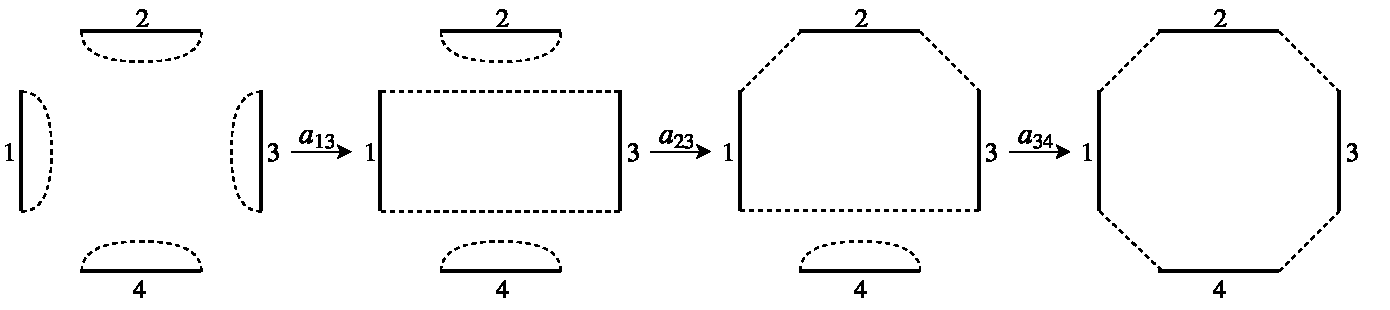
\includegraphics[width=\linewidth]{img/merge-into-cycle.pdf}
    \caption{Пример объеденения в цикл длины $4$}
    \label{merge-into-cycle}
\end{figure}

Отметим, что для наглядности, подписывая номера на блоках, мы имеем ввиду номера на соответствующих рёбрах.
Под соответствующим рёбром понимается ребро, наиболее близкое при движении по часовой стрелке.

Величина $a_{ij}$ на конкретном шаге могла получиться двумя способами: сначала выбран блок $i$, потом блок $j$, или же наоборот, $j$ потом $i$. Поэтому итоговую формулу будет необходимо домножить на $2^{m-1}$, так как всего шагов $m-1$.

Далее заметим, что для объединения в цикл не важен порядок операций, в котором они стоят. То есть сценарий $a_{13}, a_{23}, a_{34}$ равен сценарию $a_{23}, a_{13} a_{34}$ с точностью до перестановки. Следовательно, мы можем не учитывать конкретный порядок операций, а просто запоминать их множество, при этом домножив формулу на число перестановок, равное $(m-1)!$.

Полученный объект можно интерпретировать как множество рёбер в соответствующем остовном дереве. Пример подобного соответствия представлен на рис. ~\ref{tree-bijection}.
\begin{figure}[h!]
    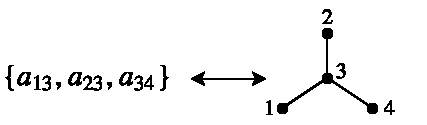
\includegraphics[width=3in]{img/tree-bijection.pdf}
    \caption{Пример биекции с остовными деревьями}
    \label{tree-bijection}
\end{figure}

Как известно, остовные деревья в графе размера $m$, кодируются кодами Прюфера \cite{prufer}, состоящими из $m-2$ чисел из множества ${1,2,\ldots,m}$. 
Нам необходимо получить сумму вероятностей по всем возможным сценариям слияния фиксированных блоков в цикл длины $m$, мы свели эту задачу к сумме по всем остовным деревьям размера $m$.
Степень вершины интерпретируется как число раз, когда соответствующее ребро было вовлечено в перестройку.
Теперь можно воспользоваться обобщенной формулой Кэли \cite{cayley}:
$$ \sum_T \prod_{i=0}^m p_i^{d_i(T)} 
= p_1 \ldots p_m (p_1 + \ldots + p_m) ^ {m - 2} \, . $$
С учётом возможных перестановок получим итоговую формулу:
$$2 ^ {m - 1} (m - 1)! p_1 \ldots p_m (p_1 + \ldots + p_m) ^ {m - 2} \, .$$

Важно отметить, что ввиду устройства операции ДРС, вероятности на рёбрах могут меняться.
Но для объединения в цикл нас интересует только сумма вероятностей в компоненте, а не отдельные $p_i$.
В процессе перераспределения сумма весов остаётся неизменной, а значит, наши рассуждения остаются верными.
\end{proof}

\subsection{Вычисление многомерного интеграла}
\begin{lemma}
$$
    \idotsint_{ \mathbb{R}^m_+} {
        \alpha_1 \cdot \ldots \cdot \alpha_m
        (\alpha_1 + \ldots + \alpha_m) ^ {m - 2}
        e ^ { -\sum_{i=1}^{m} ((\gamma + 1) \alpha_i)}
        \mathrm{d} \alpha_1 \ldots \mathrm{d} \alpha_m
    } = $$ $$ =  \frac
    {(3 m - 3)!}
    {(2 m - 1)! (\gamma + 1) ^ {3 m - 2}}
    \label{l-int}.
$$
\end{lemma}

\begin{proof}
Введём замену $t_i = \alpha_i (\gamma + 1)$:
$$
    \idotsint_{ \mathbb{R}^m_+} {
        \frac {t_1} {\gamma + 1} \cdot \ldots \cdot \frac {t_m} {\gamma + 1}
        \left(\frac {t_1 + \ldots + t_m} {\gamma + 1}\right) ^ {m - 2}
        e ^ { -\sum_{i=1}^{m} t_i}
        \frac {\mathrm{d} t_1} {\gamma + 1} \ldots \frac {\mathrm{d} t_m} {\gamma + 1}
    } = $$ $$ = \frac 1 {(\gamma + 1)^{3m-2}}
    \idotsint_{ \mathbb{R}^m_+} {
        t_1 \cdot \ldots \cdot t_m
        (t_1 + \ldots + t_m) ^ {m - 2}
        e ^ { -\sum_{i=1}^{m} t_i}
        \mathrm{d} t_1 \ldots \mathrm{d} t_m
    }
$$
Введём замену $u = t_1 + \ldots + t_m$:
$$
    \frac 1 {(\gamma + 1)^{3m-2}}
    \intop_{0}^{\infty}
    \idotsint_{ \sum_{i=1}^{m-1} t_i \leq u} {
        t_1 \ldots t_{n-1}
        \left(u - \sum_{i=1}^{m-1} t_i\right)
        u ^ {m - 2}
        e ^ {-u}
        \mathrm{d} t_1 \ldots \mathrm{d} t_{m-1} \mathrm{d} u
    } = $$ $$
    = \frac 1 {(\gamma + 1)^{3m-2}}
    \left(
        \intop_{0}^{\infty}
        \idotsint_{ \sum_{i=1}^{m-1} t_i \leq u} {
            t_1 \cdot \ldots \cdot t_{m-1}
            u ^ {m - 1}
            e ^ {-u}
            \mathrm{d} t_1 \ldots \mathrm{d} t_{m-1} \mathrm{d} u
        } -
        \right. $$ $$ \left. % hack for nice brackets
        - (m - 1)
        \intop_{0}^{\infty}
        \idotsint_{\sum_{i=1}^{m-1} t_i \leq u} {
            t_1^2 \cdot t_2 \cdot \ldots \cdot t_{m-1}
            u ^ {m - 2}
            e ^ {-u}
            \mathrm{d} t_1 \ldots \mathrm{d} t_{m-1} \mathrm{d} u
        }
    \right) = $$ $$
    = \frac 1 {(\gamma + 1)^{3m-2}}
    \left(
        \intop\nolimits_{0}^{\infty}
        \left(
            \idotsint_{ \sum_{i=1}^{m-1} t_i \leq u} {
                t_1 \cdot \ldots \cdot t_{m-1}
                \mathrm{d} t_1 \ldots \mathrm{d} t_{m-1}
            }
        \right)
        u ^ {m - 1}
        e ^ {-u}
        \mathrm{d} u
        \right. $$ $$ \left. % hack for nice brackets
        - (m - 1)
        \intop\nolimits_{0}^{\infty}
        \left(
            \idotsint_{ \sum_{i=1}^{m-1} t_i \leq u} {
                t_1^2 \cdot t_2 \cdot \ldots \cdot t_{m-1}
                \mathrm{d} t_1 \ldots \mathrm{d} t_{m-1}
            }
        \right)
        u ^ {m - 2}
        e ^ {-u}
        \mathrm{d} u
    \right) =
$$
$$ = \textrm{[по лемме ~\ref{subint1} и лемме ~\ref{subint2}]} = $$
$$
    = \frac 1 {(\gamma + 1)^{3m-2}}
    \left(
        \intop\nolimits_{0}^{\infty}
        \frac {u ^ {3m - 3} e ^ {-u}} {(2m - 2)!}
        \mathrm{d} u
        - (m - 1)
        \intop\nolimits_{0}^{\infty}
        \frac {2 u ^ {3m - 3} e ^ {-u}} {(2m - 1)!}
        \mathrm{d} u
    \right)
    = $$ $$ =
    \frac 1 {(\gamma + 1)^{3m-2}}
    \left(
        \frac 1 {(2m - 2)!}
        - \frac {2 (m - 1)} {(2m - 1)!}
    \right)
    \intop\nolimits_{0}^{\infty} u ^ {3m - 3} e ^ {-u} \mathrm{d} u
    = $$ $$ =
    \frac 1 {(\gamma + 1)^{3m-2}}
    \left(
        \frac {2m - 1 - 2m + 2} {(2m - 1)!}
    \right)
    \Gamma(3m-2)
    =
    \frac
    {(3 m - 3)!}
    {(2 m - 1)! (\gamma + 1) ^ {3 m - 2}}
$$
\end{proof}

\begin{lemma}
$$
    \idotsint_{ \sum_{i=1}^{n} t_i \leq u} {
        t_1 \cdot \ldots \cdot t_{n}
        \mathrm{d} t_1 \ldots \mathrm{d} t_{n}
    } =
    \frac {u ^ {2n}} {(2n)!}
    \label{subint1}.
$$
\end{lemma}
\begin{proof}
Доказательство проведём по индукции. База индукции, $n = 1$:
$$
    \intop_0^u {t \mathrm{d} t} =
    \frac {u ^ 2} 2 - \frac {0 ^ 2} 2 =
    \frac {u ^ 2} 2
$$
Шаг индукции, пусть выполняется:
$$
    \idotsint_{ \sum_{i=1}^{n} t_i \leq u} {
        t_1 \cdot \ldots \cdot t_{n}
        \mathrm{d} t_1 \ldots \mathrm{d} t_{n}
    } =
    \frac {u ^ {2n}} {(2n)!} \, .%точка
$$
Вычислим:
$$
    \idotsint_{ \sum_{i=1}^{n+1} t_i \leq u} {
        t_1 \cdot \ldots \cdot t_{n+1}
        \mathrm{d} t_1 \ldots \mathrm{d} t_{n+1}
    } =
    \intop_{0}^{u}
    \frac {(u - t_{n+1})^{2n}} {(2n)!} t_{n+1}
    \mathrm{d} t_{n+1}
    = $$ $$ =
    - \frac 1 {(2n)!}
    \intop_{0}^{u}
    t_{n+1} \mathrm{d} \left(\frac {(u - t_{n+1})^{2n + 1}} {2n + 1}\right)
    = $$ $$ =
    - \frac 1 {(2n)!}
    \left( \left.
        \frac {(u - t_{n+1})^{2n + 1} t_{n+1}} {2n + 1} \right|_0^u
        - \intop_{0}^{u}
        \frac {(u - t_{n+1}) ^ {2n+1}} {2n+1}
        \mathrm{d} t_{n+1}
    \right)
    = $$ $$ =
    \frac 1 {(2n + 1)!}
    \intop_{0}^{u}
    (u - t_{n+1}) ^ {2n+1}
    \mathrm{d} t_{n+1}
    =
    \frac 1 {(2n + 1)!}
    \left( \left.
        - \frac
        {(u - t_{n+1}) ^ {2n+2}}
        {2n + 2}
        \right|_0^u
    \right)
    = $$ $$ =
    \frac {u ^ {2n+2}} {(2n + 2)!}
$$
\end{proof}

\begin{lemma}
$$
    \idotsint_{ \sum_{i=1}^{n} t_i \leq u} {
        t_1^2 \cdot t_2 \cdot \ldots \cdot t_{n}
        \mathrm{d} t_1 \ldots \mathrm{d} t_{n}
    } =
    \frac {2 u ^ {2n + 1}} {(2n + 1)!}
    \label{subint2}.
$$
\end{lemma}
\begin{proof}
Доказательство проведём по индукции. База индукции, $n = 1$:
$$
    \intop_0^u {t^2 \mathrm{d} t} =
    \frac {u ^ 3} 3 - \frac {0 ^ 3} 3 =
    \frac {u ^ 3} 3
$$
Шаг индукции, пусть выполняется:
$$
    \idotsint_{ \sum_{i=1}^{n} t_i \leq u} {
        t_1^2 \cdot t_2 \cdot \ldots \cdot t_{n}
        \mathrm{d} t_1 \ldots \mathrm{d} t_{n}
    } =
    \frac {2 u ^ {2n + 1}} {(2n + 1)!}
$$
Вычислим:
$$
    \idotsint_{ \sum_{i=1}^{n+1} t_i \leq u} {
        t_1 \cdot t_2 \cdot \ldots \cdot t_{n+1}
        \mathrm{d} t_1 \ldots \mathrm{d} t_{n+1}
    } =
    \intop_{0}^{u}
    \frac {2 (u - t_{n+1})^{2n + 1}} {(2n + 1)!} t_{n+1}
    \mathrm{d} t_{n+1}
    =
$$ $$
    = - \frac 2 {(2n + 1)!}
    \intop_{0}^{u}
    t_{n+1} \mathrm{d} \left(
        \frac {(u - t_{n+1})^{2n + 2}} {2n + 2}
    \right)
    =
$$ $$
    =
    - \frac 2 {(2n + 1)!}
    \left( \left.
        \frac {(u - t_{n+1})^{2n + 2} t_{n+1}} {2n + 2} \right|_0^u
        - \intop_{0}^{u}
        \frac {(u - t_{n+1}) ^ {2n+2}} {2n+2}
        \mathrm{d} t_{n+1}
    \right)
    = $$ $$ =
    \frac 2 {(2n + 2)!}
    \intop_{0}^{u}
    (u - t_{n+1}) ^ {2n+2}
    \mathrm{d} t_{n+1}
    =
    \frac 2 {(2n + 2)!}
    \left( \left.
        - \frac
        {(u - t_{n+1}) ^ {2n+3}}
        {2n + 3}
        \right|_0^u
    \right)
    = $$ $$ =
    \frac {2 u ^ {2n+3}} {(2n + 3)!} \, .%точка
$$
\end{proof}


\section{Построение метода оценки истинного эволюционного расстояния}
Для оценки истинного эволюционного расстояния будем использовать кумулятивные статистики.
Первая статистика $\frac b n$ --- это нормированное число нетривиальных циклов:
$$\frac b n = 1 - \frac {c_1} n = 1 - \frac 1 {1 + \gamma} = \frac \gamma {1 + \gamma} \, .%точка 
$$

Вторая статистика $\frac d n$ --- это нормированнное минимальное эволюционное расстояние.
$$\frac d n = \sum_{m=2}^{\infty} \frac {c_m} n (m-1) =
1 - \frac
{(1 + \gamma)^2 ({}_2F_1\left(-\frac 2 3, -\frac 1 3, \frac 1 2, \frac {27 \gamma} {4 (1 + \gamma)^3}\right) - 1)}
{3 \gamma} \, .%точка
$$

Чтобы оценить истинное эволюционное расстояние, узнаем реальные $d$ и $b$ на текущем геноме.
Так как функция $\frac d b$ непрерывна и монотонна, мы можем найти её корень простым двоичным поиском, тем самым, мы узнаём $\gamma$.
Далее, зная $\gamma$, находим значение $\frac b n$.
Для того, чтобы предсказать $n$, достаточно разделить $b$ на $\frac b n$.
Всё что осталось --- вспомнить, что $k = \frac {\gamma n} 2$.

В листинге ~\ref{lst} приведен код данного метода на языке \textit{Python 3}:
\begin{algorithm}[!h]
\caption{Алгоритм оценки истинного эволючионного расстояния}
\label{lst}
\begin{lstlisting}[language=Python]
def predict_k(d, b):
    d_over_n = lambda x: 1 - (1 + x) ** 2 * (hyp2f1(-2 / 3, -1 / 3, 1 / 2, 27 * x / (4 * (1 + x) ** 3)) - 1) / (3 * x)
    b_over_n = lambda x: x / (1 + x)
    d_over_b = lambda r: lambda x: d_over_n(x) / b_over_n(x) - r

    gamma = optimize.bisect(d_over_b(d / b), 1e-6, 3, xtol=1e-4)
    b_n = b_over_n(gamma)
    n = b / b_n
    return n * gamma / 2
\end{lstlisting}
\end{algorithm}

Далее, проведём симуляции геномных перестроек на языке \textrm{Python} и оценим работу алгоритма для $\gamma \in [0,5, 2.0)$. Граница парсимонии находится на $\gamma = 0,5$, поэтому меньшие значения нас не интересуют. $\gamma \geq 2$ не рассматриваются, так как настолько удаленные геномы очень редки.

Для оценки работы алгоритма построен график распределения относительной ошибки $\frac {k_e - k} k$ от $\gamma$ вида <<ящик с усами>>. <<Ящикам>> соответсвуют $50 \, \%$ результатов, <<усам>> соответствуют $90 \, \%$. График приведен на рис. ~\ref{dir_est_05_20}. Как мы видим, $50 \, \%$ результатов оценки ошибаются не более, чем на $6 \, \%$, а $90 \, \%$ результатов ошибаются не более, чем на $10 \, \%$. Что является хорошим показателем для оценки в рамках модели.
\begin{figure}[h!]
    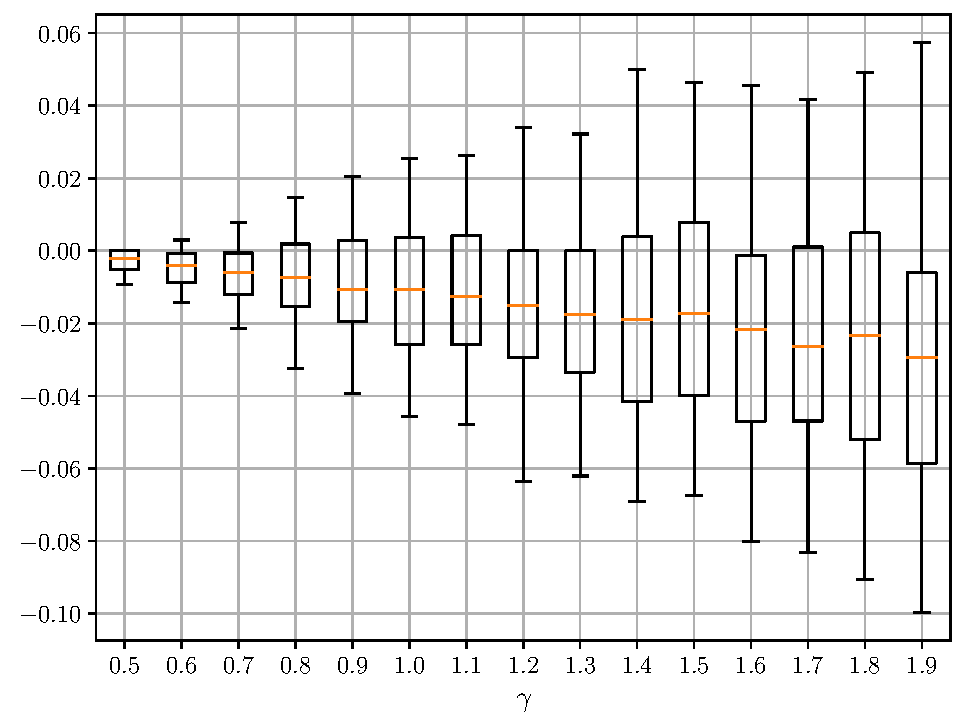
\includegraphics[width=0.8\linewidth]{img/dir_est_05_20.pdf}
    \caption{Зависимость распределения относительной ошибки $\frac {k_e - k} k$ от $\gamma$ в новом методе оценки}
    \label{dir_est_05_20}
\end{figure}

Также, в таблице ~\ref{tab-est-error} приведено соответствие среднего модуля ошибки $\frac {k_e - k} k$ в процентах от $\gamma \in [0,5, 2.0)$.

\begin{table}[!h]
  \caption{Средний модуль ошибки в процентах в зависимости от $\gamma$}\label{tab1}
  \centering
  \begin{tabular}{|*{4}{c|}}\hline
  \( \gamma \) & Средний модуль ошибки & \( \gamma \) & Средний модуль ошибки \\\hline
  $0.5$ & $0.3 \, \%$ & $1.3$ & $2.78 \, \%$ \\\hline
  $0.6$ & $0.58 \, \%$ & $1.4$ & $3.12 \, \%$ \\\hline
  $0.7$ & $0.86 \, \%$ & $1.5$ & $3.14 \, \%$ \\\hline
  $0.8$ & $1.24 \, \%$ & $1.6$ & $3.57 \, \%$ \\\hline
  $0.9$ & $1.59 \, \%$ & $1.7$ & $3.76 \, \%$ \\\hline
  $1.0$ & $1.88 \, \%$ & $1.8$ & $4.02 \, \%$ \\\hline
  $1.1$ & $2.1 \, \%$ & $1.9$ & $4.49 \, \%$ \\\hline
  $1.2$ & $2.43 \, \%$ & $2.0$ & $4.87 \, \%$ \\\hline
  \end{tabular}
  \label{tab-est-error}
\end{table}
%!!! я проглядел этот момент -- обычно смотрят на средний квадрат  ошибки, а не модуль. Но сейчас уже не меняйте

Как видно из рис. ~\ref{dir_est_05_20}, в данном методе оценки присутствует систематическая ошибка (предсказанное $k$ в среднем оказывается меньше, чем реальное).
Это связано с тем, что асимптотические оценки учитывают только компоненты первого порядка.
Но цикл заданной длины иногда может получаться ввиду распада цикла большей длины.

Для того, чтобы учесть этот факт, эмпирически оценим данную погрешность и учтём её.
Для $\gamma < 0.5$ погрешность для $\frac{d}{n}$ равняется $0$, а для $\gamma \geq 0.5$ она составляет $\frac{0.1}{\sqrt{n}}$.
Результаты работы метода оценки, учитывающего данную погрешность приведены на рис. ~\ref{dir_est_05_20_buffed}.
\begin{figure}[h!]
    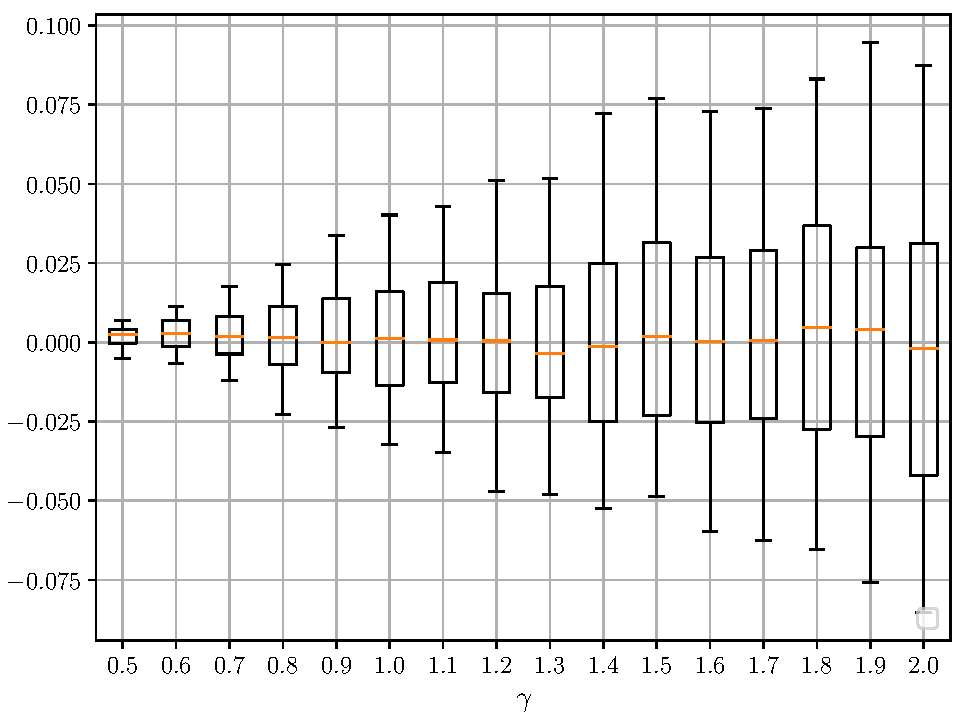
\includegraphics[width=0.8\linewidth]{img/dir_est_05_20_buffed.pdf}
    \caption{Зависимость распределения относительной ошибки $\frac {k_e - k} k$ от $\gamma$ в новом методе оценки с учетом эмпирической оценки на погрешность}
    \label{dir_est_05_20_buffed}
\end{figure}

\chapterconclusion
В главе 2 проведён теоретический анализ модели Дирихле и произведена асимптотическая оценка всех необходимых компонент, построены комбинаторные формулы для среднего числа компонент в общем случае. 

Предложен новый метод оценки истинного эволюционного расстояния в рамках этой модели, а также описана его реализация. Проведена оценка точности работы метода для $\gamma \in [0,5, 2.0)$.